% THIS IS SIGPROC-SP.TEX - VERSION 3.1
% WORKS WITH V3.2SP OF ACM_PROC_ARTICLE-SP.CLS
% APRIL 2009

\documentclass{acm_proc_article-sp}

\newcommand{\superscript}[1]{\ensuremath{^{\textrm{#1}}}}
\def\sharedaffiliation{\end{tabular}\newline\begin{tabular}{c}}

\def\wu{\superscript{1}}
\def\wg{\superscript{2}}



\usepackage{url}
\usepackage{color}
\usepackage{multirow}
\usepackage{mathtools}

\begin{document}

%\title{Context-aware Connections between News Events}
\title{Describing and Contextualizing News Events in TV}
%\subtitle{Exploring DBpedia paths between named entities belonging to different event contexts}

\numberofauthors{5} 

\author{
\alignauthor
Laurens De Vocht\wu
       \affaddr{\email{\texttt{laurens.devocht@ugent.be}}}
\and
\alignauthor
Erik Mannens\wu
       \affaddr{\email{\texttt{erik.mannens@ugent.be}}}
\and
\alignauthor
Rik Van de Walle\wu
       \affaddr{\email{\texttt{rik.vandewalle@ugent.be}}}
% 3rd. author
\and
\alignauthor 
Rapha\"el Troncy\wg
	\affaddr{\email{\texttt{raphael.troncy@eurecom.fr}}}
\and
\alignauthor 
Jos\'e Luis Redondo Garc\'ia\wg
	\affaddr{\email{\texttt{redondo@eurecom.fr}}}
\sharedaffiliation
\begin{tabular}{ccc}
    \affaddr{{\wu}Ghent University - iMinds - Multimedia Lab{\ }} & & 
    \affaddr{{\wg}EURECOM{\ }} \\
    %\affaddr{Gaston Crommenlaan 8/201} & \affaddr{} \\
    \affaddr{Ghent, Belgium} & &
    \affaddr{Biot, France} \\
\end{tabular}
}
%USED SHARED AFFILIATIONS TO SAVE SPACE

\maketitle
\begin{abstract}
There exist many approaches tackling the challenge of finding relevant entities to a document, but : 
(i) there are not mentioned;
(ii) there are not ranked
(iii) there are not related.
%TODO: Can you explain these a bit more?
In this paper we combine the power of non-structured resources with structured resources of DBpedia. Many applications and users leverage these entities to construct and link to other media.
We demonstrate that ... by explaining a use case about ...
%TODO: complete after the use case is written out.

\end{abstract}

% A category with the (minimum) three required fields
%\category{H.4}{Information Systems Applications}{Miscellaneous}
%A category including the fourth, optional field follows...
%\category{D.2.8}{Software Engineering}{Metrics}[complexity measures, performance measures]

%\terms{Theory}

%\keywords{ACM proceedings, \LaTeX, text tagging} % NOT required for Proceedings

\section{Introduction}

Online media is increasing in scale and ubiquity, but it is currently still unstructured and not good connected to media of other forms or from other sources.
[State of the Art: Named Entity Extraction, Expansion]
First attempts for extracting named entities out of media, which is a more and more common practice, give promising results but there it introduces some issues.
%TODO: Go deeper in these issues: probably related to those mentioned in the abstract.
LinkedTV is an integrated and practical approach towards experiencing Networked Media in the Future Internet. Within LinkedTV we want to connect media based on extracted entities that we link to DBpedia resources.

[More about LinkedTV?]
%TODO: Add here more info about the project

%[State of the Art: Everything is Connected]
We use therefore an optimized pathfinding algorithm \cite{de2013discovering} implemented in the Everything is Connected Engine (EiCE), firstly introduced with the Everything is Connected (EiC) Demo at the \emph{ISWC`12 Boston} conference.
Applying these algorithms to Linked Data can facilitate the resolving of complex queries that involve the semantics of the relations between resources. This method makes it is possible not only to discover relevant resources but also to filter them adapted to a specific context. Users can control and define which kinds of connections and types of resources really matter. Each path path between the discovered resources has a semantic meaning can be traced back to the original configuration of the user and
forms the basis of an explanation rather than a ranking. A major contribution in this approach is that it minimizes the size of the candidate pool of nodes in order to optimize queries and increase
the quality of the resulting paths.

\section{The Approach}

The approach described in this paper intends to reconstruct the semantic context associated to one particular news video, highlighting the main concepts and entities involved and explaining how they are related to each other. The complete processing workflow takes as input the textual transcript of a multimedia resource depicting the event, as well as the start and end date for which that particular event has been considered relevant. If the event is still ongoing we consider the current day as the end of the temporal interval. The corresponding video providers and platforms make sure this data is available beforehand.

In addition, we assume that the analyzed event has a minimum presence and coverage in the Web in order to ensure that the subsequent data mining techniques can collect an enough quantity of data to reconstruct the event's context. The output of the algorithm is a pair $Context_{Event1}=\left [  \varepsilon , \rho \right ]$  where $\varepsilon$ is a list named entities together with a numeric relevance score ($ \varepsilon =\left \{ E\times \mathbb{R} \right \}$,  being $E$ named entities classified using the NERD ontology\footnote{\url{http://nerd.eurecom.fr/ontology/nerd-v0.5.n3}}) and $\rho$ is a set of predicates $\left [ e_{1},e_{2}, p \right ]$, relating the aforementioned entities ($e_{1}\in E \vee  e_{2}\in E$). 

Our hypothesis states that this knowledge representation of the events can provide a sufficient source of information for satisfying the viewer's information needs and supporting complex multimedia operations such as search and hyperlinking. In the following subsections we further explain the logic for entity expansion as illustrated in Figure~\ref{fig:namedEntityExpansion}.

\begin{figure}[h!]
\centering
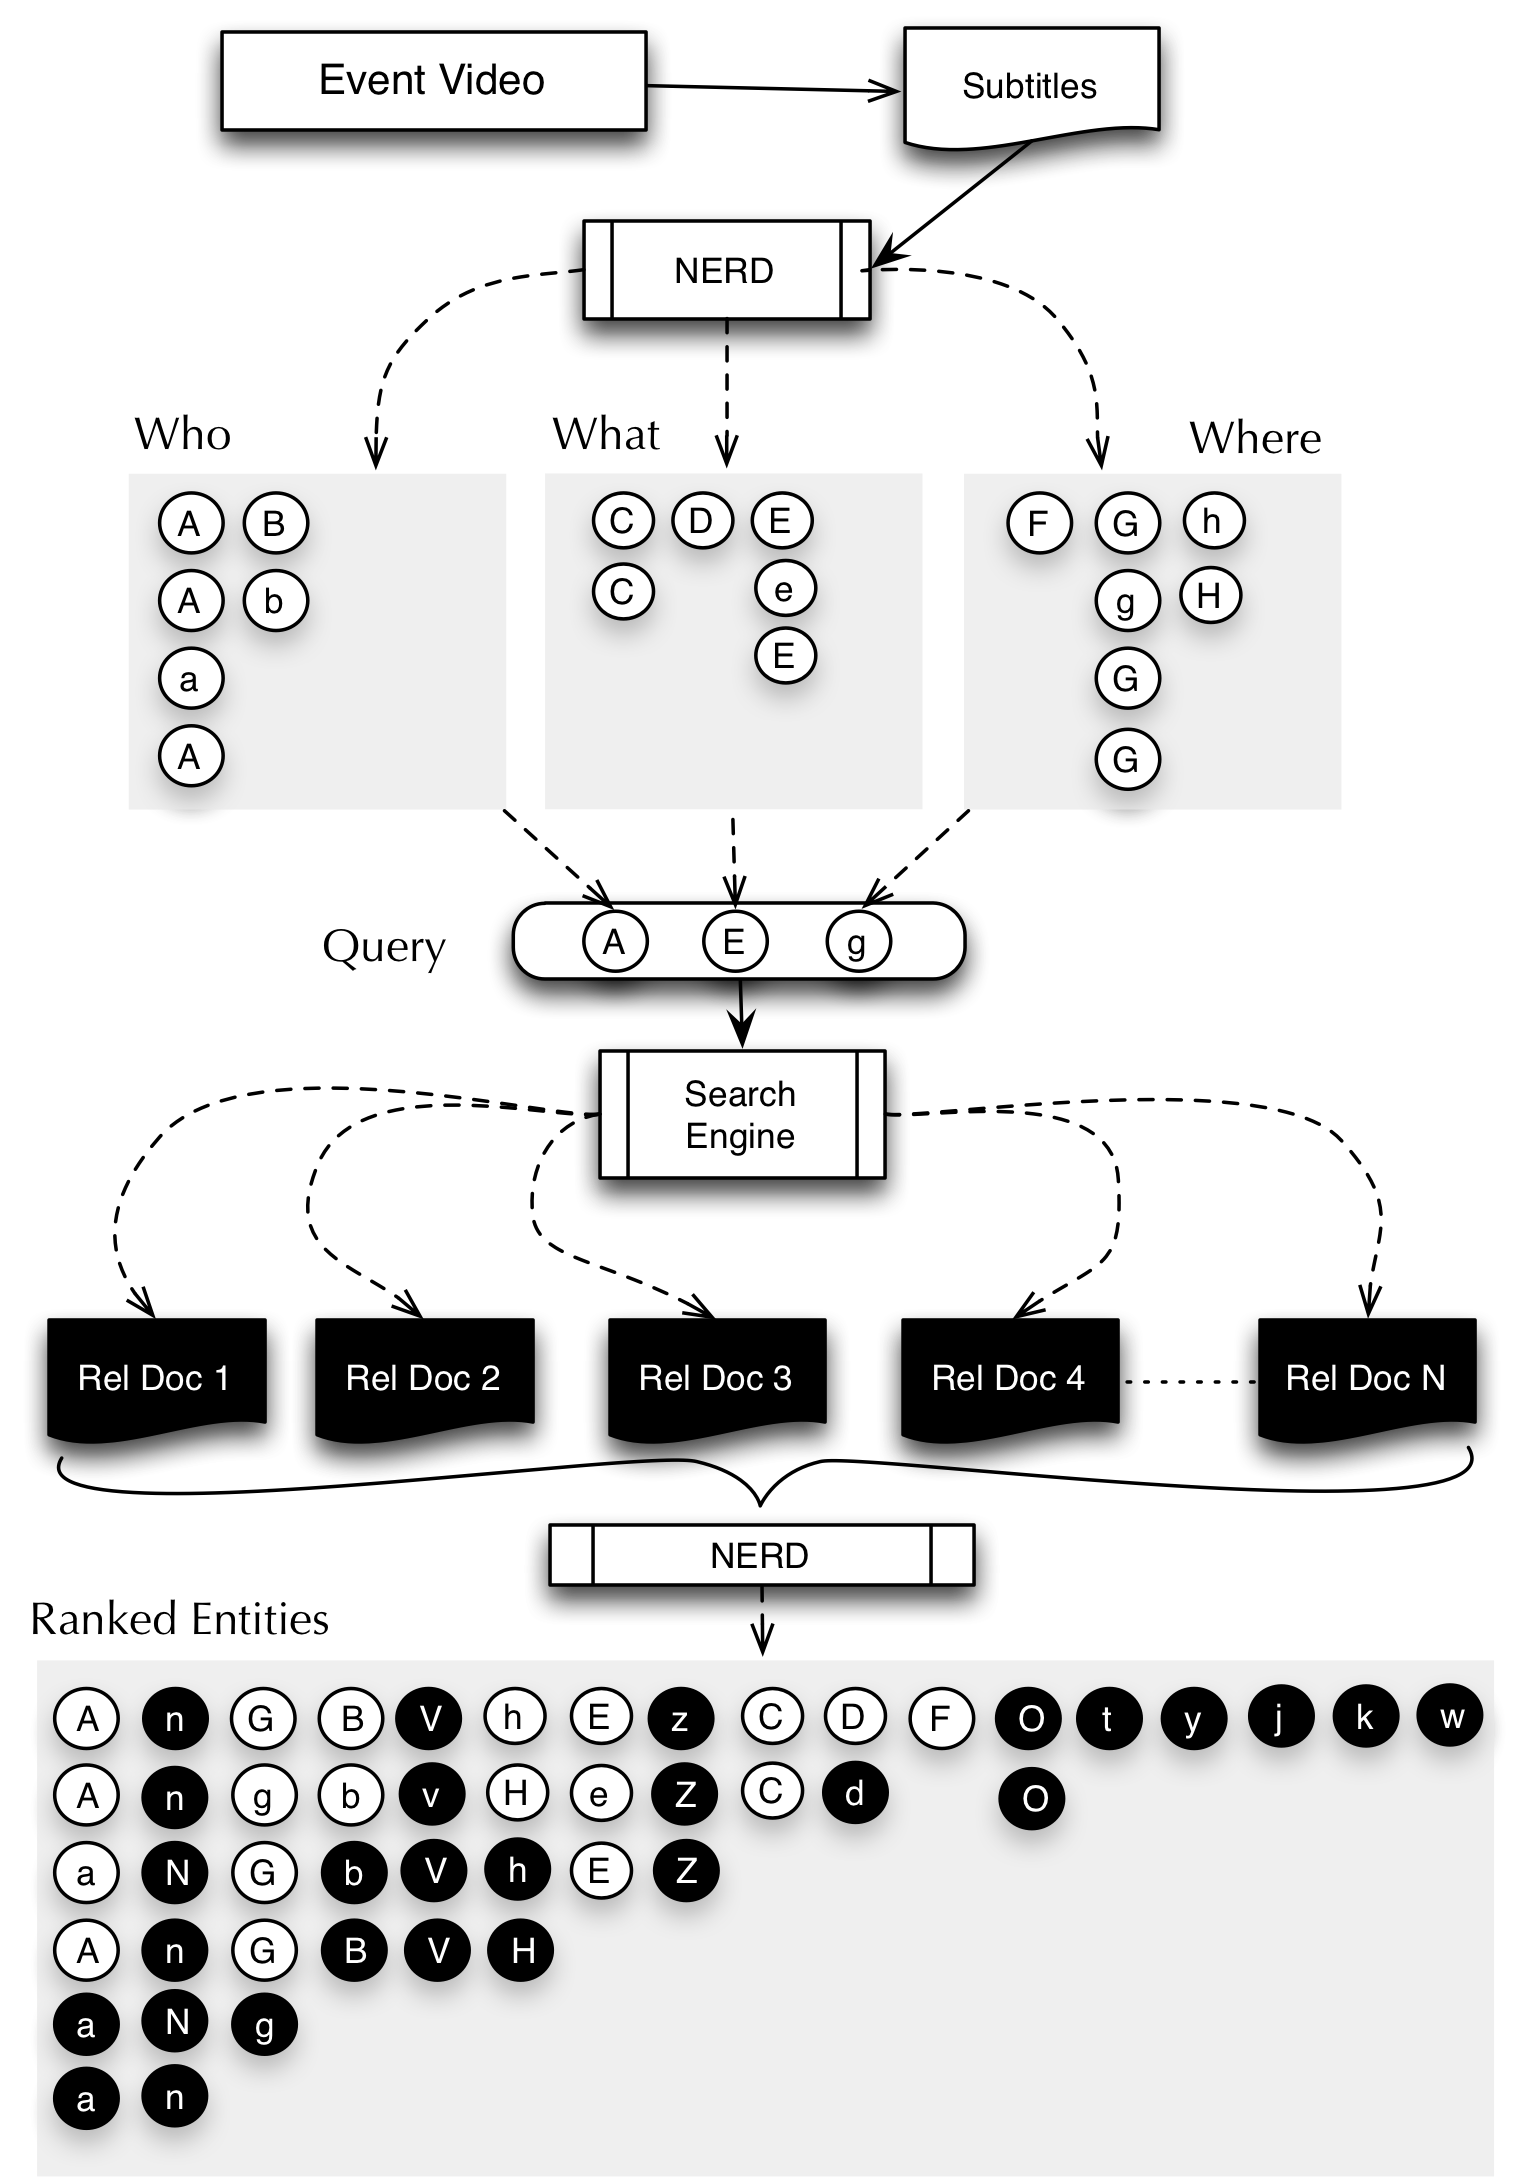
\includegraphics[width=0.4\textwidth]{figure/ExpansionDiagram}
\caption{Schema of Named Entity Expansion Algorithm.}
\label{fig:namedEntityExpansion}%\end{figure}
\end{figure}

\subsection{Named Entity Extraction}

For each news item we perform named-entity recognition over the corresponding subtitles by using the NERD~\cite{Rizzo2012b} framework. The language of the considered videos is English but NERD supports many other languages so our approach is applicable in other languages. The output of this phase is a collection of entities annotated using the NERD Ontology v0.5, that come with a first relevance score obtained from the considered extractors. This set includes a first set of ranked entities that are explicitly mentioned during the video. Even there are still missing entities that can be relevant for the viewer in the context of the current event, this is where other video description approximations~\cite{yunjia2013} stop. However, for us this will be a first list of concepts to be used as base for the entity expansion component.

\subsection{Context through Expansion}

Expand the context by identifying named entities in the media fragments.

Motivation: Bigger view. 

Graphic.

Output.

\subsubsection{Query Generation}

The who what where method [reference]

The Five Ws is a popular concept for information gathering in journalistic reporting.
It captures all aspects of a story or incidence: who, when, what, where, and why.
We propose a framework composed of a suite of cooperating visual information displays to represent the Five Ws and demonstrate its use within a healthcare informatics application. 

This is somewhat like what a school child does when learning to write a descriptive sentence of the event. It is taught that one should pay attention to the 5 W�s \cite{LiJia2007}: who, where, what, when and how. In our system, we try to answer 3 of the 5 W�s: what (the event label), where (the scene en- vironment label) and who (a list of the object categories).

Map to the NERD model
First textual query

\subsubsection{Document retrieval}

Temporal reference, is a function of the time of the event. Different nature of the events, different nature of the search engine. we consider. this. 

Google search

The quality of the search

\subsubsection{Entity fusion}

Logic for entity. Cluster. 
Centroid of the cluster/URL.

Future: Semantic in wordnet.

\subsubsection{Entity Ranking}

Considered features for ranking

Formula applied

Output is a list of entities. Normally filtered because there are many.

\subsection{Generating DBpedia paths}

Entities are divided in two groups: main entities, and tail.

Before we filter the relations between resources, the candidate resources to be included in relations are being pre-ranked. They are pre-ranked according to ``popularity'' and ``rarity'' essential components in the original PageRank algorithm \cite{page1999pagerank} and is used to sort candidate related nodes in the EiCE. The implementation of the EiCE takes the relations in to account by making use of the Jaccard coefficient to measure the dissimilarity and assign random walks based weight able to highly rank more rare resources, guaranteeing that paths between resources prefer specific relations and not general ones \cite{moore2012novel}.

\begin{figure}[h!]
\centering
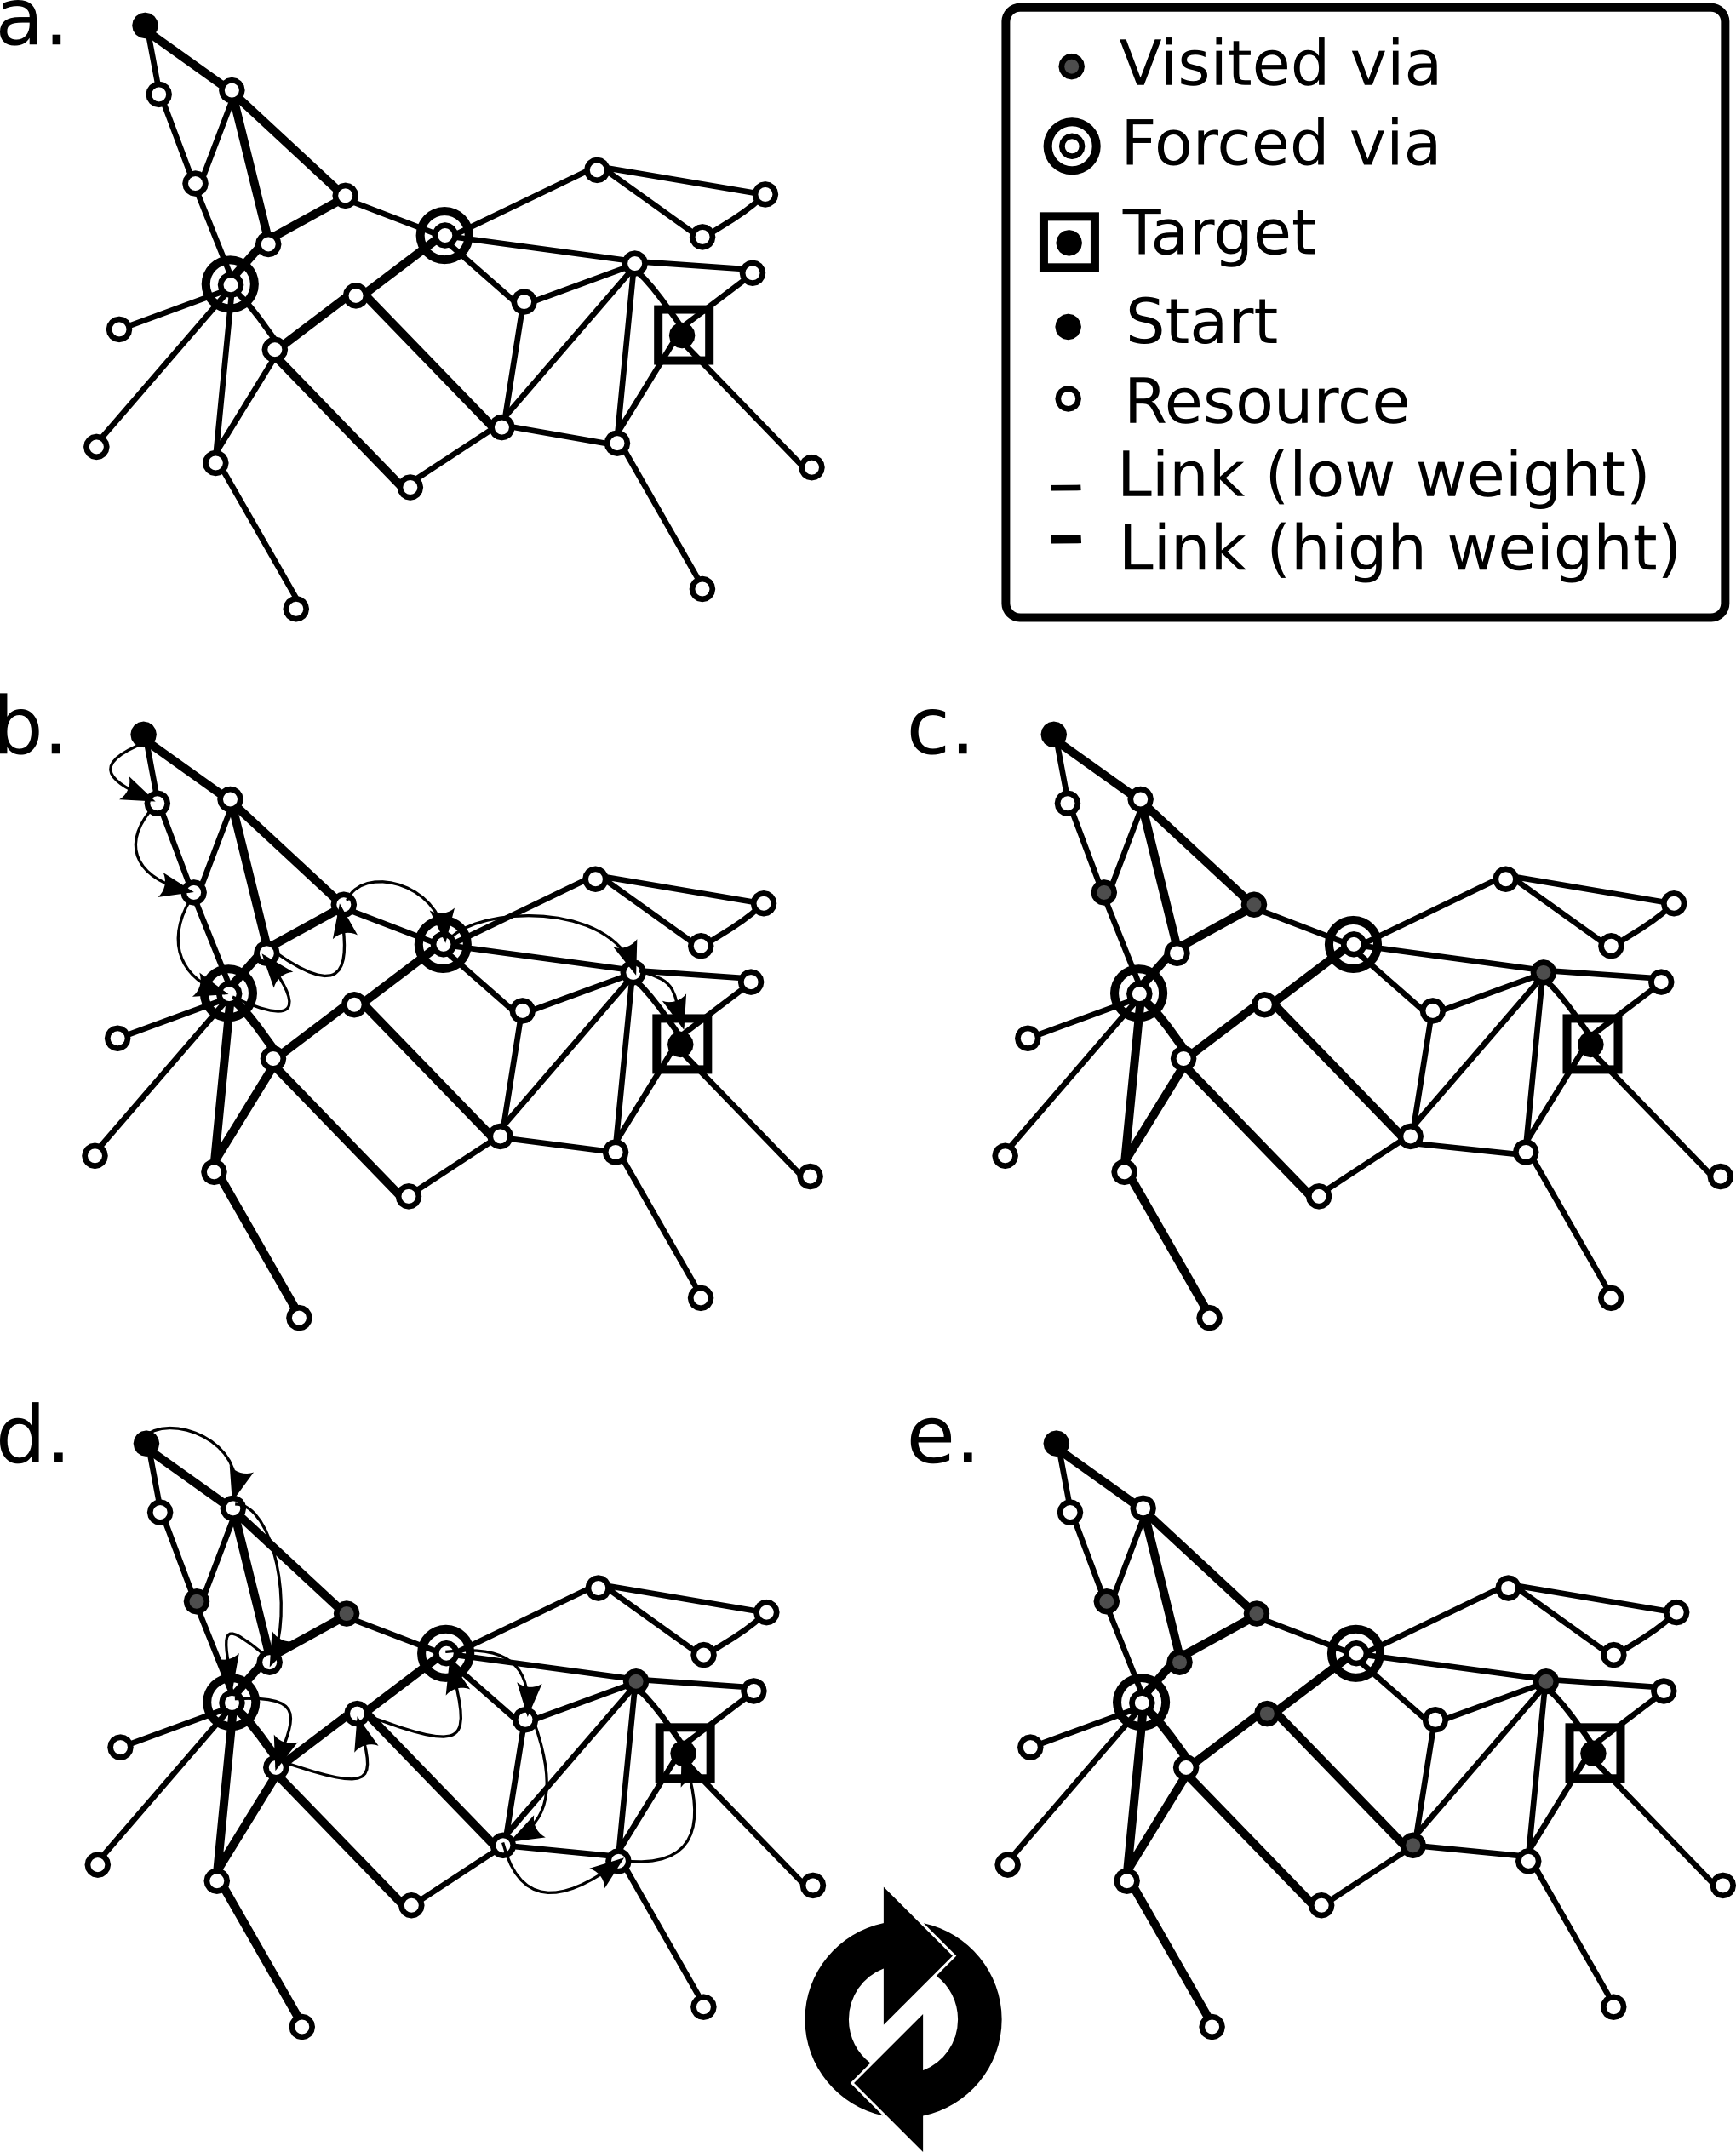
\includegraphics[width=0.4\textwidth]{graphmultipatternmatching.png}
\caption{Pattern matching with multiple results using an iterative pathfinding process.}
\label{fig:patternmatching}
\end{figure}

We pass on the main start resource, a target and via points. Figure~\ref{fig:patternmatching} shows the iterative process for generating DBPedia paths. An initial state is computed in step \ref{fig:patternmatching}a. There are low weights and high weights, for the example 1 and 2 respectively. Based on the weights of the links te path through the vias is optimized, so a path with the lowest total weight will be selected first, until the vias are added to the exclude list. The path from start to end is forced through the given via points (\ref{fig:patternmatching}b). This leads to additional visited resource as via points (\ref{fig:patternmatching}c). They occur because to resolve each path, the route is being computed starting in the start resource, target and the via points. The resources where they converge to each other are considered as the new via points. These via points are included in the paths and therefore marked as visited. This is to make sure that in the next iteration paths will go around the visited via (\ref{fig:patternmatching}d). The next paths are being computed over and over (\ref{fig:patternmatching}e) until a threshold number of paths is found , and the context is large enough or when it takes to long to compute the next path (out of range). The final set of optimized paths used to for the context expansion.

\subsection{Filtering Context Relevant Paths}

We use the current API calls with the entities we have detected and investigate what the frequent paths returned are. We count(?) the most frequently(?) occurring:
predicates and resources.

Issue: what is the most important information in the path? The via node or the edges (dbpedia properties)?

\subsection{Reranking entities and adding properties}

Out of the resulting expanded context we extract the most important(?) entities and predicates to find related media fragments.

\subsection{Refining entities via Filtering}


\subsection{Results}

\section{Use Case: Snowden Assylum}

\section{Evaluation}

\section{Conclusions}
We presented a new approach for context-aware connecting news events. Our preliminary results indicate that by exploring DBpedia paths in named entities occuring in news media. ...
%\end{document}  % This is where a 'short' article might terminate

%ACKNOWLEDGMENTS are optional
\section{Acknowledgments}
The research activities described in this paper were funded by Ghent University,
%iMinds (Interdisciplinary institute for Technology) a research institute founded by the Flemish Government,
the Institute for the Promotion of Innovation by Science and Technology in Flanders (IWT), the Fund for Scientific Research-Flanders (FWO-Flanders), and the European Union's 7th Framework Programme via the project LinkedTV (GA 287911).

%
% The following two commands are all you need in the
% initial runs of your .tex file to
% produce the bibliography for the citations in your paper.
\bibliographystyle{abbrv}
\bibliography{connectedEvents}  % sigproc.bib is the name of the Bibliography in this case
% You must have a proper ".bib" file
%  and remember to run:
% latex bibtex latex latex
% to resolve all references
%
% ACM needs 'a single self-contained file'!
%

\end{document}
